\documentclass{cskkuproject}

\titleformat{\subsection}[hang]{\normalfont\normalsize\upshape}{\thesubsection}{0.45\firstindentlength}{}
\titleformat{name=\subsection,numberless}[hang]{\normalfont\normalsize\upshape}{}{0}{}
\titleformat{\subsubsection}[hang]{\normalfont\normalsize\upshape}{\thesubsubsection}{0.45\firstindentlength}{}
\titleformat{name=\subsubsection,numberless}[hang]{\normalfont\normalsize\upshape}{}{0}{}

\usepackage{tabularx}
\usepackage[table]{xcolor}
\usepackage{multirow}
\usepackage{graphicx}
\usepackage{array}
\newcommand{\gap}{\par\vspace{0.8ex}}
\newcommand{\safeimg}[3][0.9\textwidth]{%
  \IfFileExists{images/#2}{\includegraphics[width=#1]{images/#2}}%
  {\fbox{\parbox{0.85\textwidth}{\centering\vspace{1.5cm}\textbf{[รอรูปภาพ: \detokenize{#2}]}\\ #3\vspace{1.5cm}}}}%
}

% ==========================================
% ข้อมูลโครงงาน — กรอกข้อมูลที่นี่
% ==========================================

\titleTH{การพัฒนาเว็บแอปพลิเคชันระบบแนะนำหนังสือการ์ตูนแบบหลายพฤติกรรม สำหรับการเช่าอ่าน}
\titleEN{MULTI – BEHAVIOR RECOMMENDATION WEB APPLICATION DEVELOPMENT FOR MANGA RENTAL SERVICES}

% ข้อมูลนักศึกษาคนที่ 1
\firstStudentID{663380012-6}
\firstStudentPrefixTH{นาย}
\firstStudentPrefixEN{Mr.}
\firstStudentNameTH{ณัฐพัฒน์ แสนตรี}
\firstStudentNameEN{Nattaphat Saentree}

% ข้อมูลนักศึกษาคนที่ 2
% *** ถ้าทำโครงงานคนเดียว ให้เว้นว่างไว้ทั้งหมด (เหมือนด้านล่าง) ***
% *** ถ้ามี 2 คน ให้กรอกข้อมูลเหมือนคนที่ 1 ***
\secondStudentID{663380199-4}
\secondStudentPrefixTH{นางสาว}
\secondStudentPrefixEN{Miss}
\secondStudentNameTH{การติมา คำภีร์}
\secondStudentNameEN{Karntima Khampee}

% ข้อมูลหลักสูตร
\degreeTH{วิทยาศาสตรบัณฑิต}
\degreeEN{Bachelor of Science}
\majorTH{วิทยาการคอมพิวเตอร์}
\majorEN{Computer Science}

% อาจารย์ที่ปรึกษา
\advisorTH{รศ. ดร.ปัญญาพล หอระตะ}
\advisorEN{Assoc. Prof. Punyaphol Horata, Ph.D.}

% ปีการศึกษา
\academicYearTH{2569}
\academicYearEN{2026}

% รหัสวิชา (CP354 771 = โครงงาน 1, CP354 772 = โครงงาน 2)
\courseCode{CP354 771}
\courseName{โครงงานคอมพิวเตอร์ 1}
\semester{1}

% คำสำคัญ
\keywordsTH{ระบบแนะนำข้อมูล, การกรองข้อมูลแบบหลายพฤติกรรม, Graph Convolutional Network}
\keywordsEN{Recommender System, Multi-Behavior Collaborative Filtering, Graph Convolutional Network}


\begin{document}

% ==========================================
% หน้าปก
% ==========================================
% คำสั่งด้านล่างสร้างหน้าปกอัตโนมัติจากข้อมูลที่กรอกด้านบน
% ไม่ต้องแก้ไขส่วนนี้
\maketitlepage

% ตั้งค่าเลขหน้าส่วนต้นเป็นอักษรไทย (ก, ข, ค, ...)
\pagenumbering{arabic}
\setcounter{page}{0}
\renewcommand{\thepage}{\ThaiAlph{\value{page}}}

% ==========================================
% บทคัดย่อ
% ==========================================
\begin{abstractTH}
% บทคัดย่อภาษาไทย
% หมายเหตุ: ไม่ควรเกิน 300 คำ
% ควรครอบคลุม: วัตถุประสงค์ → วิธีการ → ผลลัพธ์ → การประยุกต์ใช้
%
% *** ลบข้อความตัวอย่างด้านล่างทั้งหมดแล้วเขียนบทคัดย่อของตนเอง ***

โครงงานนี้มีวัตถุประสงค์เพื่อพัฒนาเว็บแอปพลิเคชันต้นแบบสำหรับระบบแนะนำหนังสือการ์ตูนและออกแบบโมเดลระบบแนะนำที่วิเคราะห์พฤติกรรมผู้ใช้หลายรูปแบบเพื่อเพิ่มความแม่นยำในการแนะนำสำหรับการเช่าอ่านโดยประยุกต์ใช้โมเดล MB-CGCN (Multi-Behavior Collaborative Graph Convolutional Network) วิเคราะห์พฤติกรรมผู้ใช้ในหลายมิติได้แก่การคลิกอ่านเนื้อหาการเพิ่มเข้าตะกร้าและการเช่าอ่าน (พฤติกรรมเป้าหมาย) พร้อมทั้งพัฒนาเว็บแอปพลิเคชันต้นแบบเพื่อแสดงผลและทดสอบประสิทธิภาพของโมเดลและแก้ไขปัญหา Cold-Start ด้วยการให้ผู้ใช้ใหม่เลือกหนังสือการ์ตูนที่สนใจระหว่างการสมัครสมาชิกรวมถึงการอัปเดตผลการแนะนำแบบทันทีเมื่อผู้ใช้เพิ่มหนังสือลงในตะกร้าหรือคลิกอ่านเนื้อหา

โดยทำการประเมินและเปรียบเทียบประสิทธิภาพกับระบบแนะนำแบบพฤติกรรมเดียวด้วยตัวชี้วัด Ranking Metrics ได้แก่ Recall@K และ NDCG@K เพื่อวิเคราะห์ว่าการใช้ข้อมูลพฤติกรรมหลายรูปแบบช่วยลดปัญหา data sparsity และสะท้อนความสนใจของผู้ใช้ได้ดีขึ้นหรือไม่ซึ่งสามารถนำไปประยุกต์ใช้ในธุรกิจเช่าหนังสือการ์ตูนดิจิทัลเพื่อเพิ่มประสิทธิภาพการแนะนำเนื้อหาในเชิงพาณิชย์


\end{abstractTH}

\begin{abstractEN}
% ABSTRACT (English)
% Note: Should not exceed 300 words.
% Should cover: Objective, Methodology, Results, Applications
% Use Past tense for objectives and methodology
% Use Present tense for results and applications

This project aimed to develop a prototype web application for a manga rental service and to build a multi-behavior recommendation model. The MB-CGCN (Multi-Behavior Collaborative Graph Convolutional Network) model was used to analyze user behavior across three types of interactions: viewing content, adding to cart, and renting. A prototype web application was developed to display recommendation results, address the cold-start problem by letting new users select manga of interest during registration, and update recommendations in real time when users interact with content.

The model was evaluated against single-behavior baselines using Recall@K, NDCG@K, and other ranking metrics. Results show that incorporating multiple behaviors improves recommendation accuracy and helps reduce data sparsity. This approach is applicable to digital comic rental services and similar e-commerce platforms.

\end{abstractEN}

% ==========================================
% กิตติกรรมประกาศ
% ==========================================
\begin{acknowledgement}
% กิตติกรรมประกาศ
% หมายเหตุ: ไม่เกิน 1 หน้ากระดาษ
%
% *** ลบข้อความตัวอย่างด้านล่าง แล้วเขียนกิตติกรรมประกาศของตนเอง ***

โครงงานเรื่อง การพัฒนาเว็บแอปพลิเคชันระบบแนะนำหนังสือการ์ตูนแบบหลายพฤติกรรมสำหรับการเช่าอ่าน สำเร็จลุล่วงได้ด้วยความกรุณาและความช่วยเหลือจากบุคคลหลายฝ่าย

คณะผู้จัดทำขอกราบขอบพระคุณ รองศาสตราจารย์ ดร.ปัญญาพล หอระตะ อาจารย์ที่ปรึกษาโครงงาน ที่ได้ให้คำแนะนำ ข้อเสนอแนะ และคำปรึกษาอันเป็นประโยชน์อย่างยิ่งตลอดระยะเวลาการดำเนินโครงงาน ทั้งในด้านแนวคิดทางวิชาการ วิธีการดำเนินงาน และการตรวจสอบแก้ไขข้อบกพร่องต่าง ๆ จนทำให้โครงงานนี้สำเร็จลุล่วงไปได้ด้วยดี

นอกจากนี้ คณะผู้จัดทำขอขอบพระคุณคณาจารย์และบุคลากรของ วิทยาลัยการคอมพิวเตอร์ มหาวิทยาลัยขอนแก่น ที่ได้ถ่ายทอดความรู้และประสบการณ์ด้านวิทยาการคอมพิวเตอร์ ซึ่งเป็นพื้นฐานสำคัญในการพัฒนาโครงงานครั้งนี้
สุดท้ายนี้ คณะผู้จัดทำขอขอบคุณครอบครัว เพื่อน และผู้ที่มีส่วนเกี่ยวข้องทุกท่าน ที่ให้กำลังใจและสนับสนุนตลอดระยะเวลาการดำเนินโครงงาน

คณะผู้จัดทำหวังเป็นอย่างยิ่งว่าโครงงานฉบับนี้จะเป็นประโยชน์ต่อผู้ที่สนใจศึกษาเกี่ยวกับระบบแนะนำ ปัญญาประดิษฐ์ และการพัฒนาเว็บแอปพลิเคชันต่อไป


\end{acknowledgement}

% ==========================================
% สารบัญ
% ==========================================
\tableofcontents
\clearpage
\fancyhead[C]{}
\markboth{}{}
\listoffigures
\clearpage
\fancyhead[C]{}
\markboth{}{}
\listoftables
\clearpage
\fancyhead[C]{}
\markboth{}{}

% ==========================================
% สัญลักษณ์และคำย่อ (ถ้ามี — uncomment ด้านล่าง)
% ==========================================
% \begin{symbolpage}
% \input{symbols}
% \end{symbolpage}

% ==========================================
% เนื้อเรื่อง 5 บท
% ==========================================
% เริ่มนับเลขหน้าใหม่เป็นเลขอารบิก (1, 2, 3, ...)
% ไม่ต้องแก้ไขส่วนนี้
\pagenumbering{arabic}
\setcounter{page}{1}

\chapterone
\chaptertwo
\chapterthree
\chapterfour
\chapterfive

% ==========================================
% เอกสารอ้างอิง
% ==========================================
% *** ไม่ต้องแก้ไขส่วนนี้ ***
% ระบบจะดึงรายการอ้างอิงจากไฟล์ references.bib อัตโนมัติ
% ให้แก้ไขรายการอ้างอิงในไฟล์ references.bib แทน
\clearpage
\addcontentsline{toc}{chapter}{เอกสารอ้างอิง}
\makeatletter
\let\ps@plain\ps@empty
\makeatother
\bibliographystyle{ieeetr}
\bibliography{references}

% ==========================================
% ภาคผนวก
% ==========================================
% =============================
% ภาคผนวก
% =============================
% หมายเหตุ: ก่อนเริ่มภาคผนวก ระบบจะสร้างหน้าคั่นให้อัตโนมัติ
% ใช้คำสั่ง \appendiceschapter{ชื่อภาคผนวก} สำหรับแต่ละภาคผนวก
% ระบบจะกำหนดตัวอักษร ก, ข, ค ... ให้โดยอัตโนมัติ
% =============================
% ภาคผนวก ก
% =============================
\setcounter{chapter}{-1}
\appendiceschapter{ภาพหน้าจอระบบ}
\section*{ภาพหน้าจอระบบ}

ภาคผนวกนี้แสดงภาพหน้าจอการทำงานของระบบทั้งหมดที่พัฒนาขึ้น เพื่อให้เห็นภาพรวมของการออกแบบส่วนติดต่อกับผู้ใช้

\begin{figure}[H]
\centering
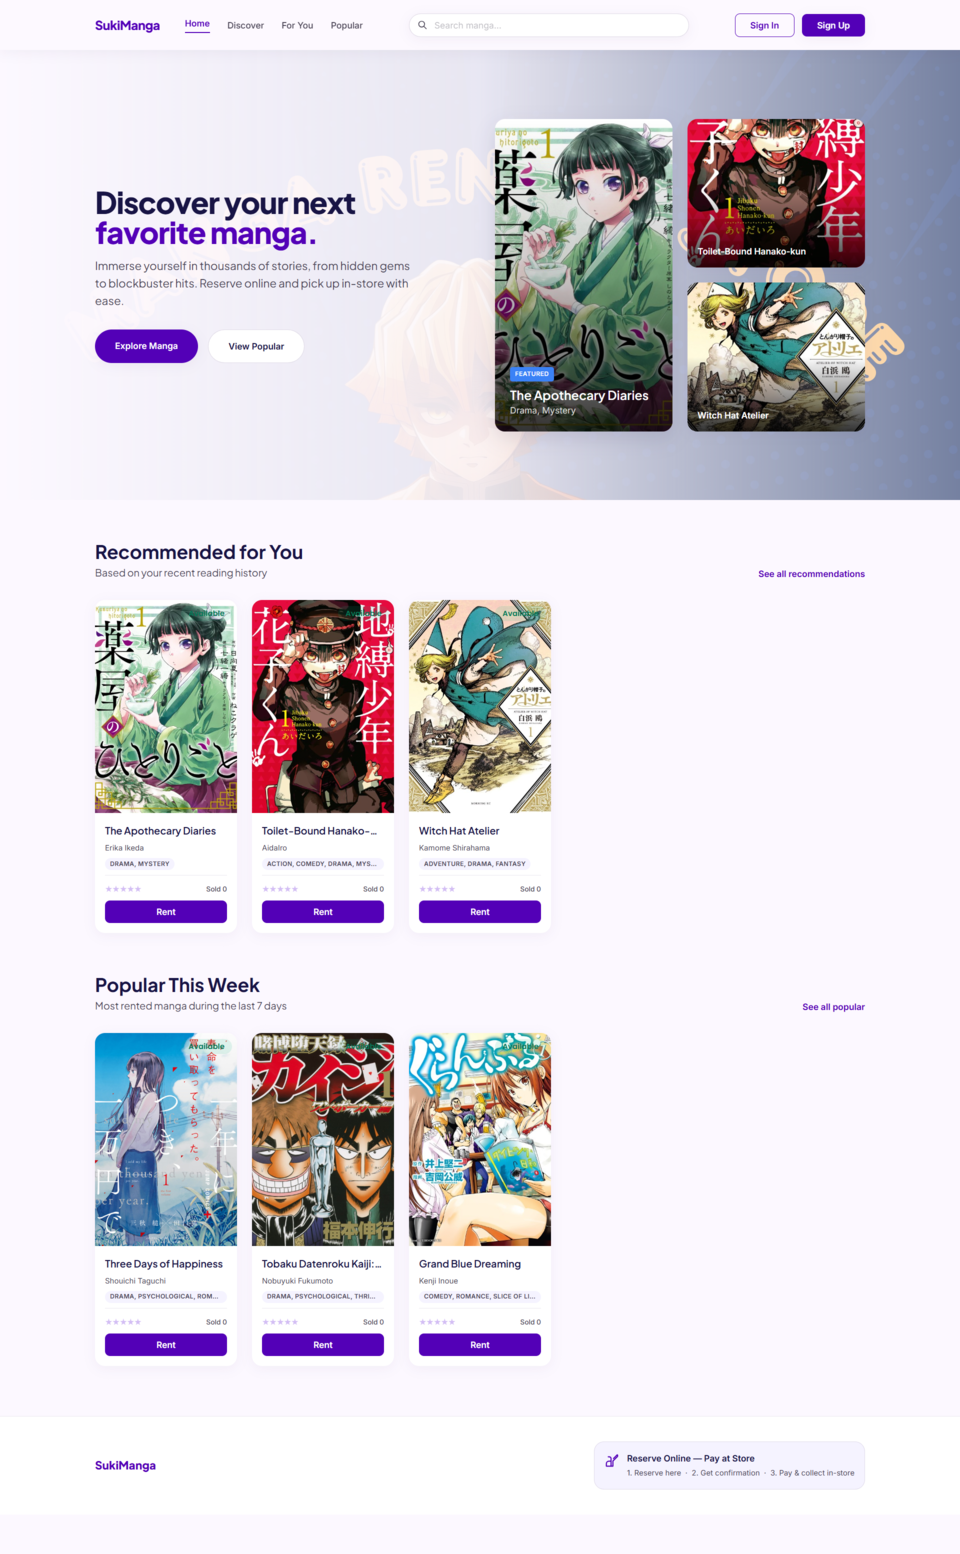
\includegraphics[width=0.8\textwidth]{images/landingPage.png}
\caption{หน้า Landing Page}
\label{fig:app_landingpage}
\end{figure}

\begin{figure}[H]
\centering
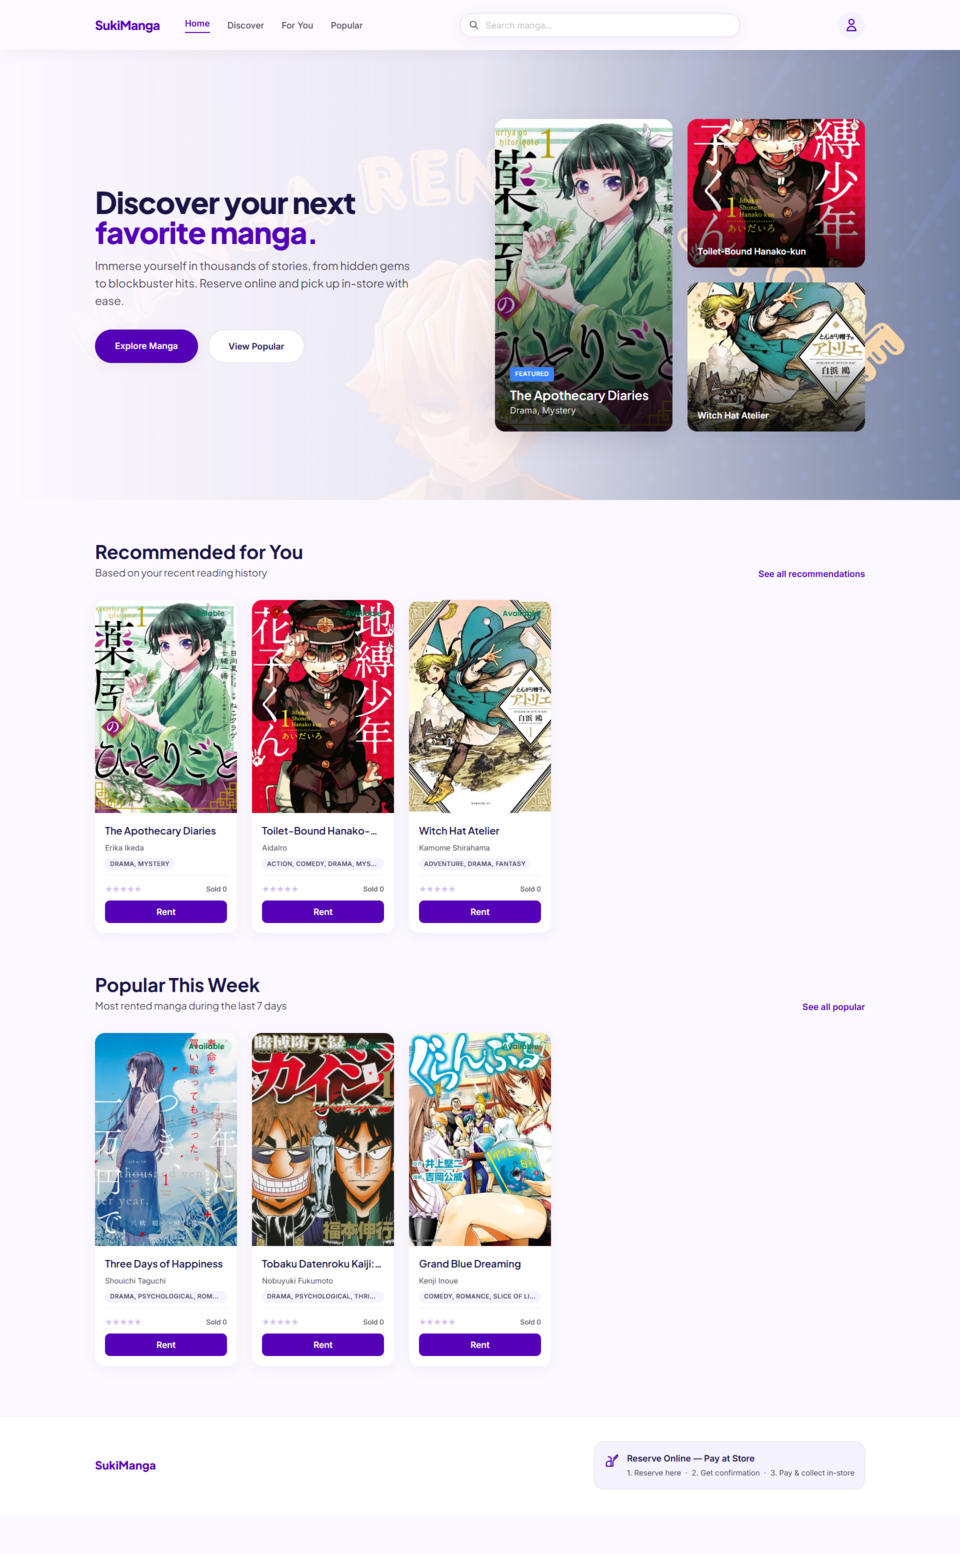
\includegraphics[width=0.8\textwidth]{images/landingPageaftersignin.png}
\caption{หน้า Landing Page หลังเข้าสู่ระบบ}
\label{fig:app_landingaftersignin}
\end{figure}

\begin{figure}[H]
\centering
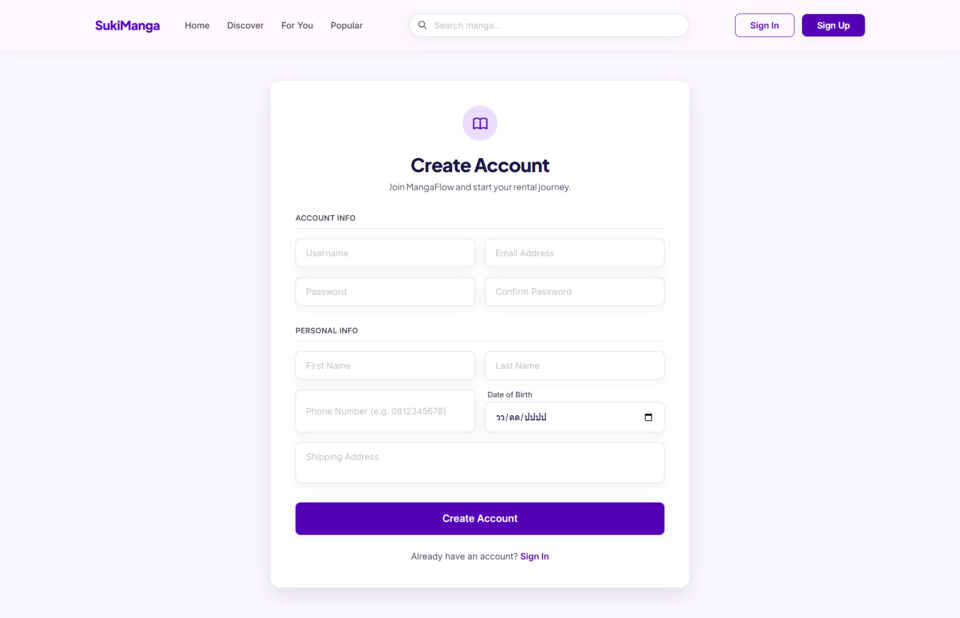
\includegraphics[width=0.8\textwidth]{images/signup.png}
\caption{หน้าสมัครสมาชิก}
\label{fig:app_signup}
\end{figure}

\begin{figure}[H]
\centering
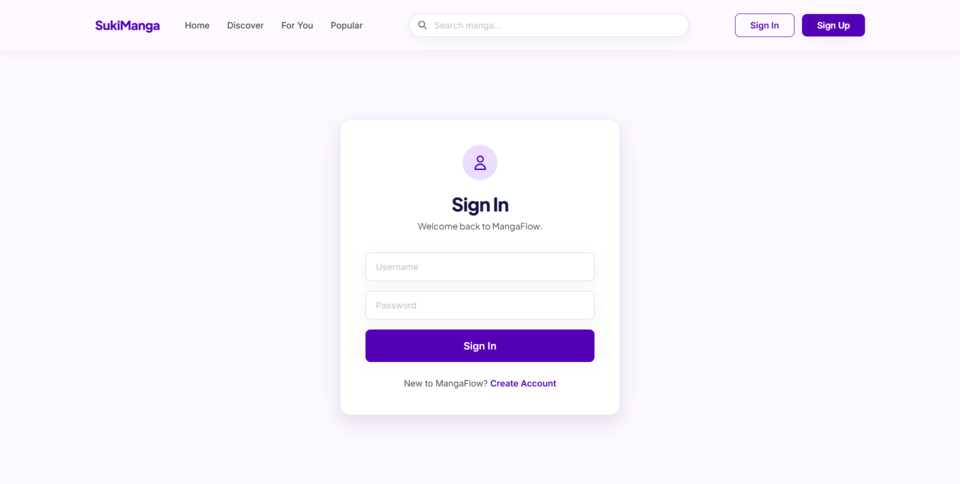
\includegraphics[width=0.8\textwidth]{images/signin.png}
\caption{หน้าเข้าสู่ระบบ}
\label{fig:app_signin}
\end{figure}

\begin{figure}[H]
\centering
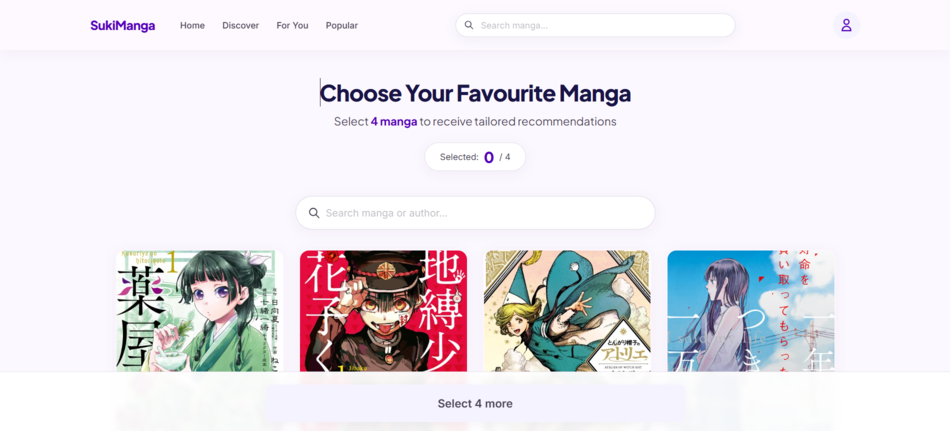
\includegraphics[width=0.8\textwidth]{images/chooseyourfav.png}
\caption{หน้าเลือกแนวการ์ตูนที่สนใจ}
\label{fig:app_chooseurfav}
\end{figure}

\begin{figure}[H]
\centering
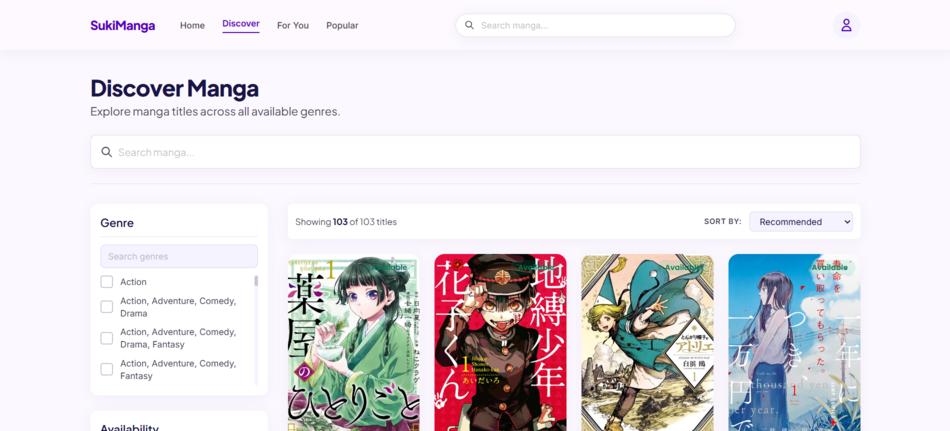
\includegraphics[width=0.8\textwidth]{images/discover.png}
\caption{หน้าค้นหาและสำรวจหนังสือ}
\label{fig:app_discover}
\end{figure}

\begin{figure}[H]
\centering
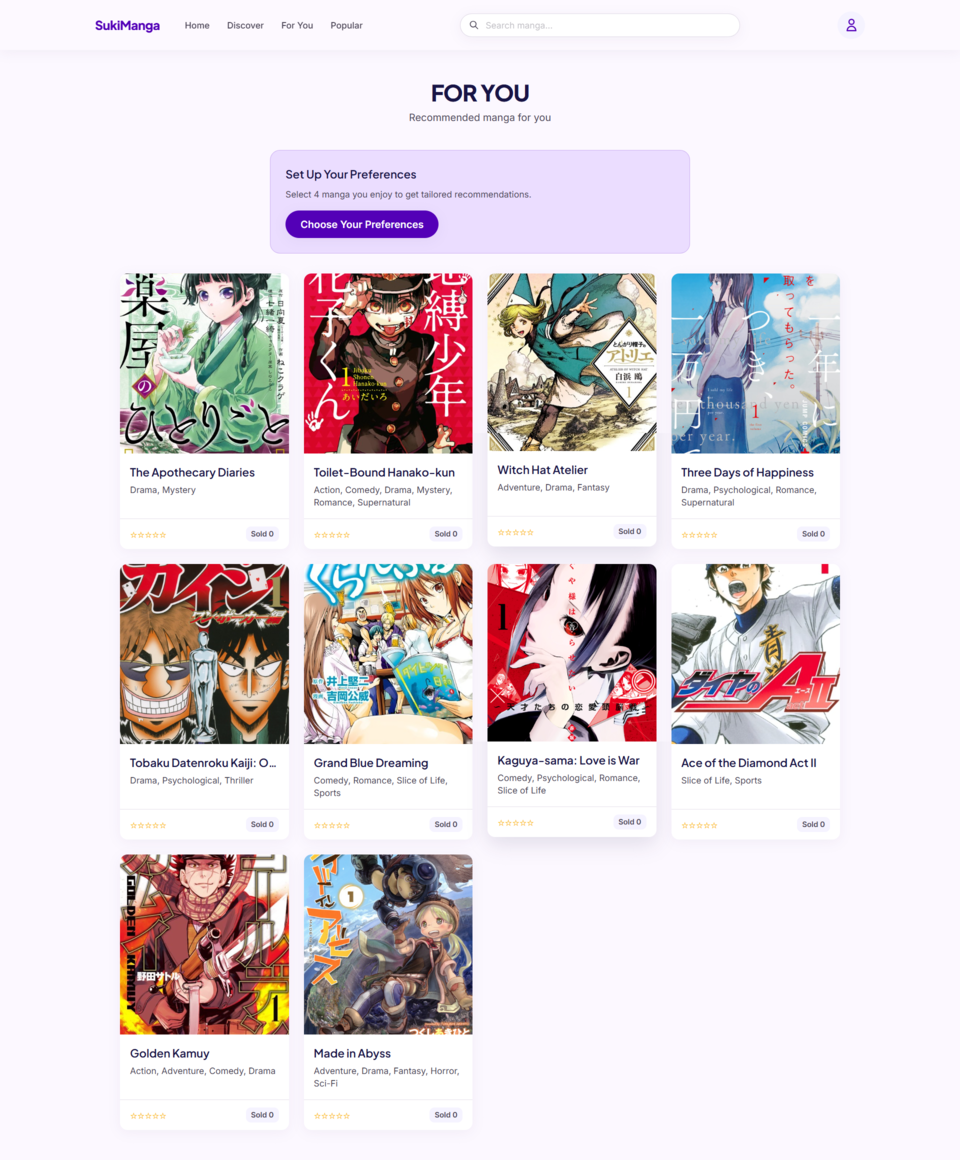
\includegraphics[width=0.8\textwidth]{images/foryou.png}
\caption{หน้าแนะนำหนังสือสำหรับคุณ}
\label{fig:app_foryou}
\end{figure}

\begin{figure}[H]
\centering
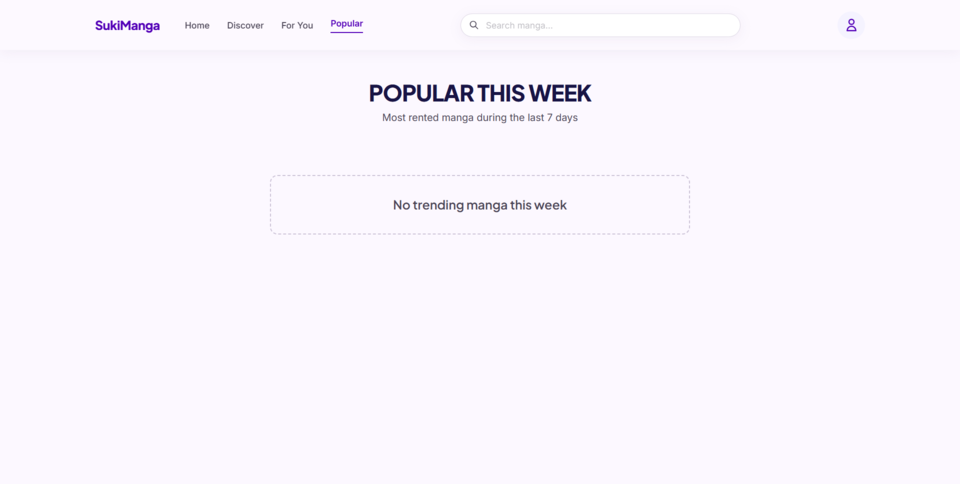
\includegraphics[width=0.8\textwidth]{images/popular.png}
\caption{หน้าหนังสือยอดนิยม}
\label{fig:app_popular}
\end{figure}

\begin{figure}[H]
\centering
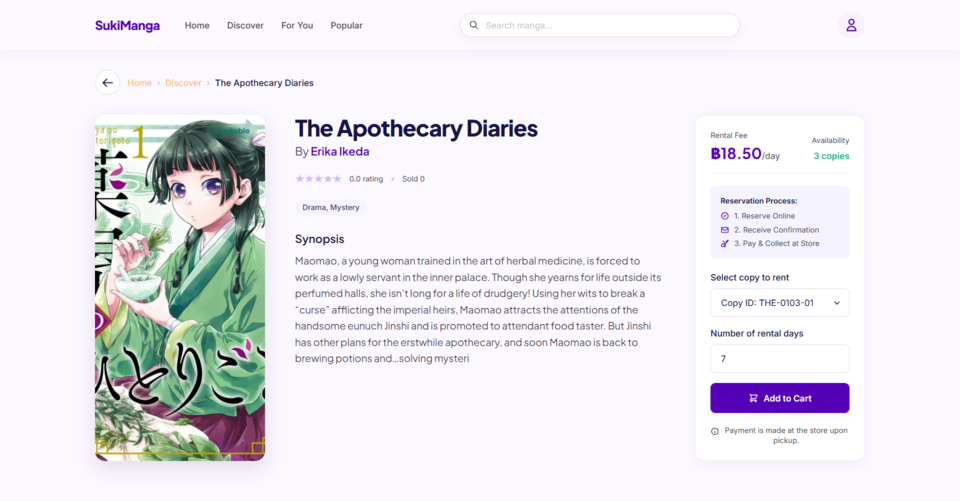
\includegraphics[width=0.8\textwidth]{images/detailManga.png}
\caption{หน้าดูรายละเอียดหนังสือ}
\label{fig:app_detailmanga}
\end{figure}

\begin{figure}[H]
\centering
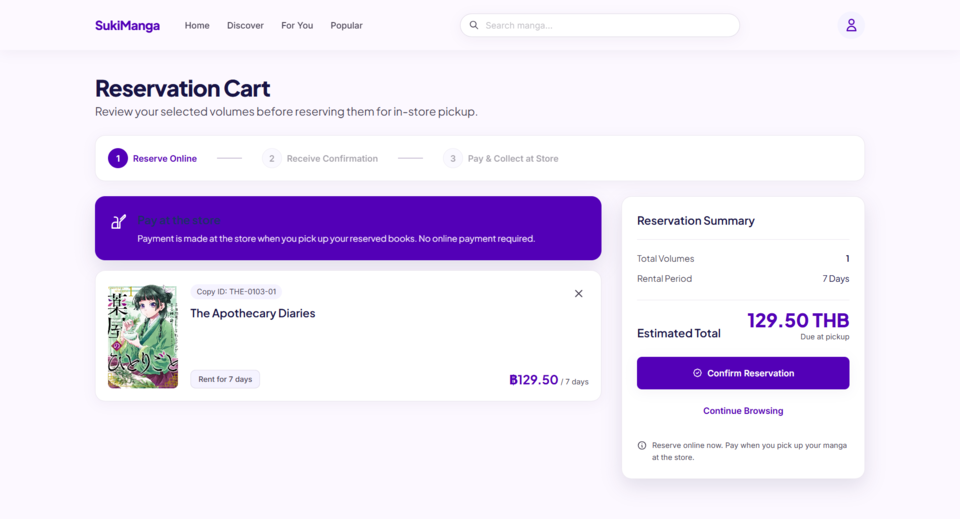
\includegraphics[width=0.8\textwidth]{images/myCart.png}
\caption{หน้าแสดงรายการที่อยู่ในตะกร้า}
\label{fig:app_mycart}
\end{figure}

\begin{figure}[H]
\centering
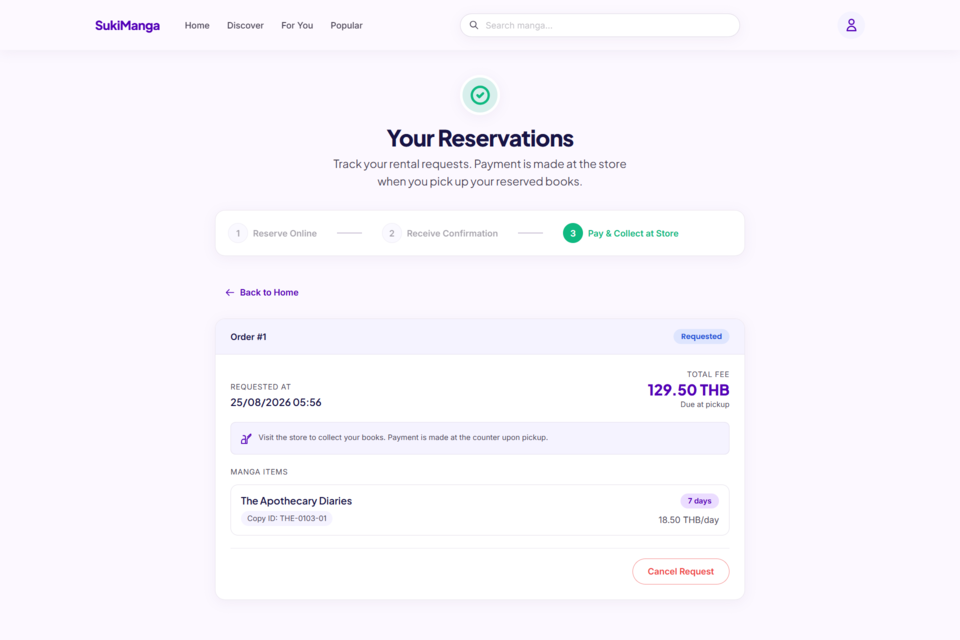
\includegraphics[width=0.8\textwidth]{images/reservationsuccess.png}
\caption{หน้าแจ้งเตือนเมื่อทำการเช่าสำเร็จ}
\label{fig:app_reservationsuccess}
\end{figure}

\begin{figure}[H]
\centering
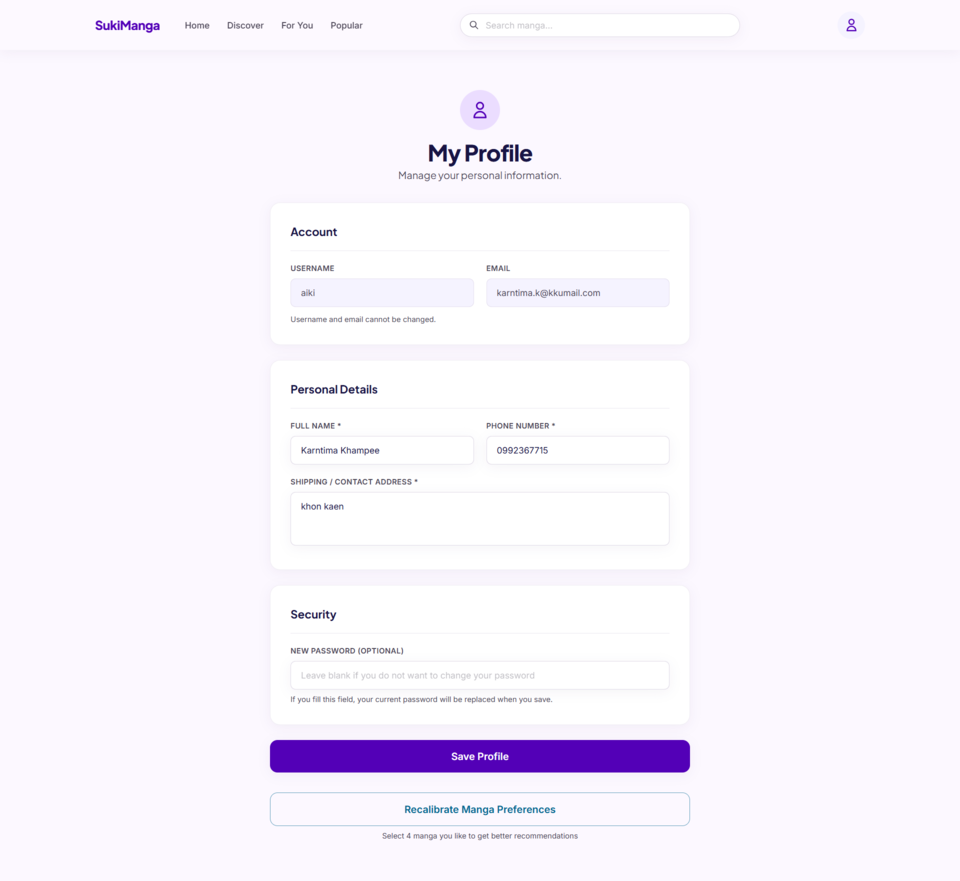
\includegraphics[width=0.8\textwidth]{images/myProfile.png}
\caption{หน้าโปรไฟล์ของผู้ใช้}
\label{fig:app_myprofile}
\end{figure}

\begin{figure}[H]
\centering
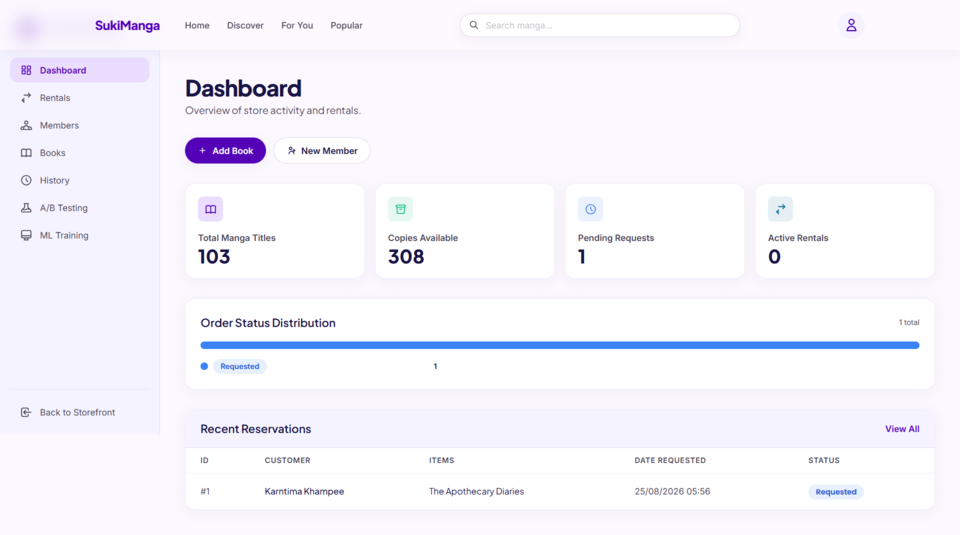
\includegraphics[width=0.8\textwidth]{images/adminDashboard.png}
\caption{หน้าแอดมิน Dashboard}
\label{fig:app_admindashboard}
\end{figure}

\begin{figure}[H]
\centering
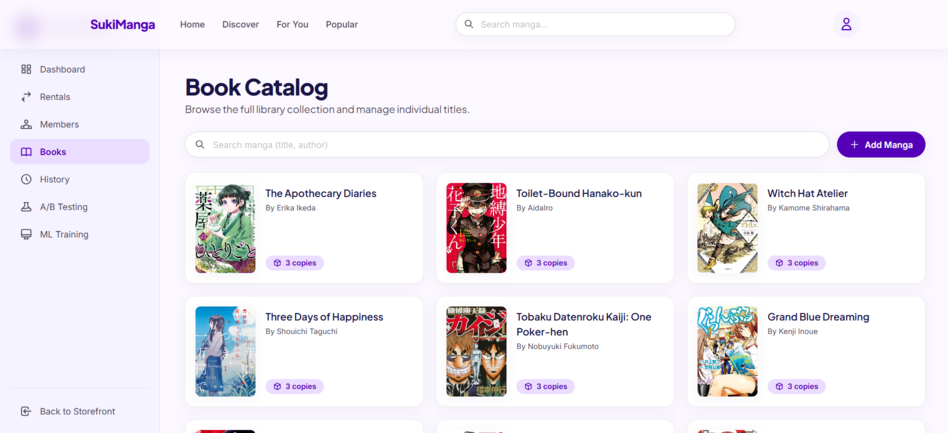
\includegraphics[width=0.8\textwidth]{images/adminManageBook.png}
\caption{หน้าจัดการรายการหนังสือ}
\label{fig:app_adminmanagebook}
\end{figure}

\begin{figure}[H]
\centering
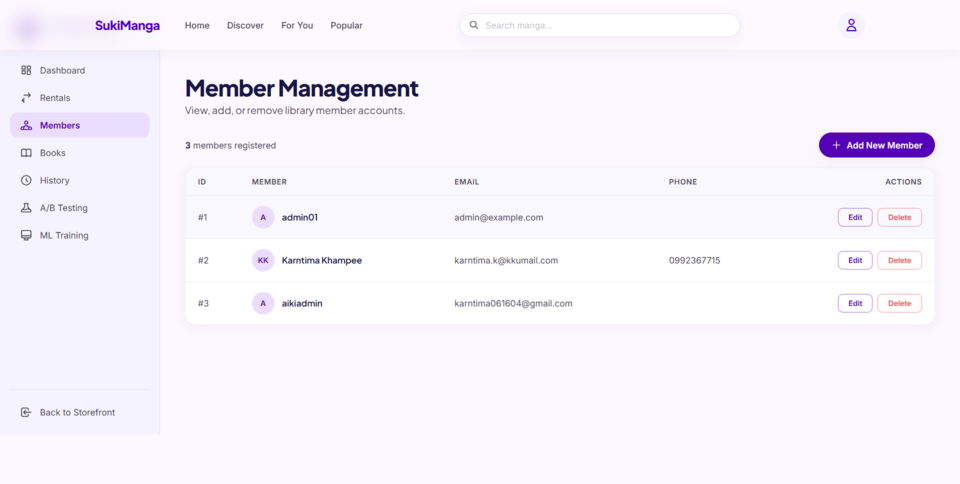
\includegraphics[width=0.8\textwidth]{images/adminManageMember.png}
\caption{หน้าจัดการสมาชิกผู้ใช้}
\label{fig:app_adminmanagemember}
\end{figure}

\begin{figure}[H]
\centering
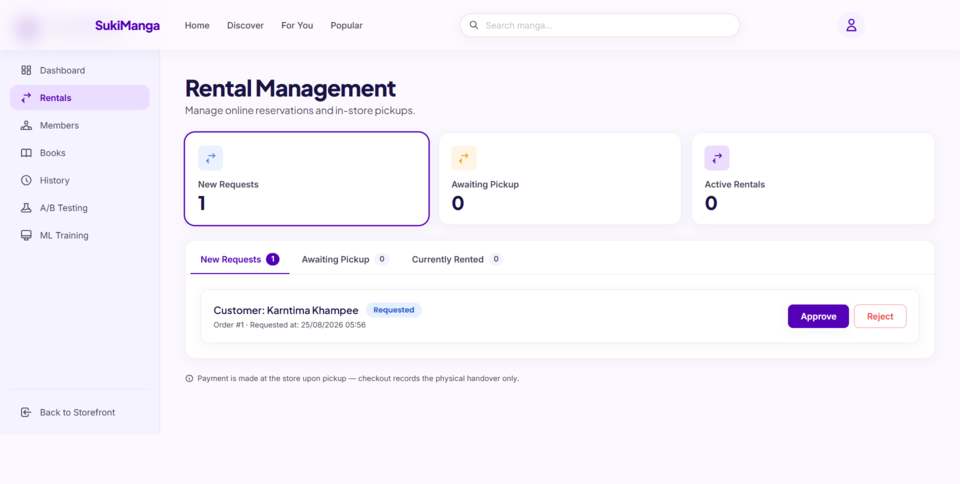
\includegraphics[width=0.8\textwidth]{images/adminManageRental.png}
\caption{หน้าจัดการรายการเช่าของแต่ละสถานะ}
\label{fig:app_adminmanagerental}
\end{figure}

\begin{figure}[H]
\centering
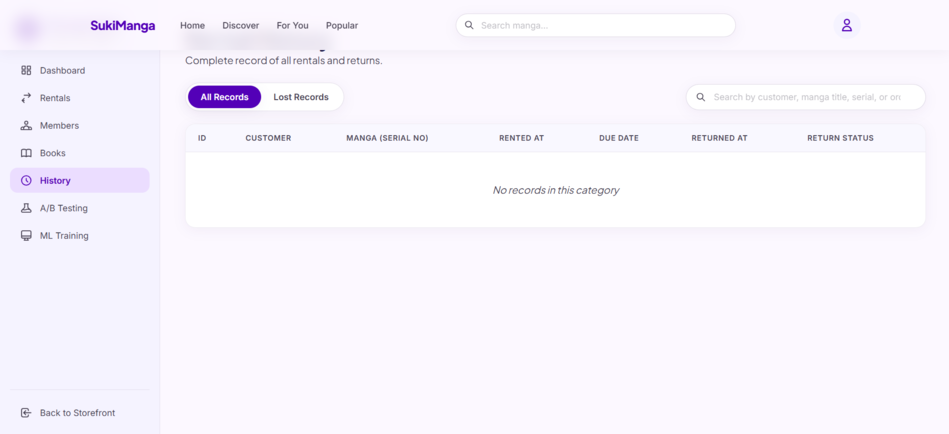
\includegraphics[width=0.8\textwidth]{images/adminViewHistory.png}
\caption{หน้าแสดงประวัติการเช่า}
\label{fig:app_adminviewhistory}
\end{figure}

\begin{figure}[H]
\centering
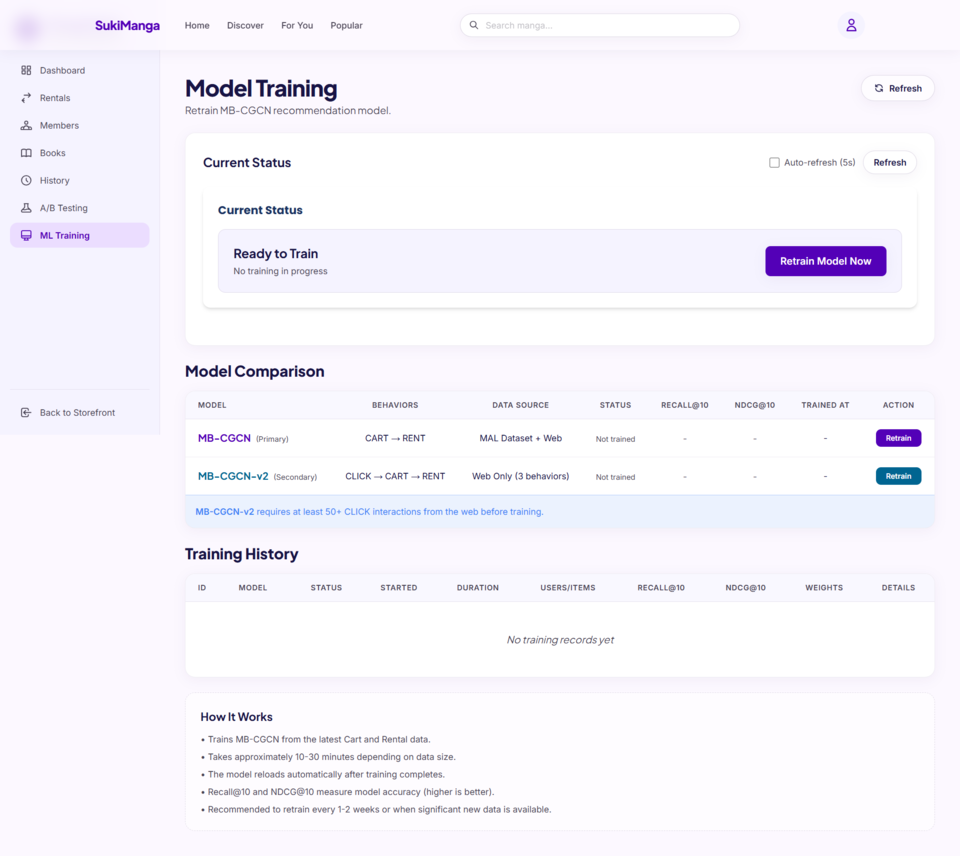
\includegraphics[width=0.8\textwidth]{images/adminMLTraining.png}
\caption{หน้าฝึกสอนโมเดลระบบแนะนำ}
\label{fig:app_adminmltraining}
\end{figure}

\begin{figure}[H]
\centering
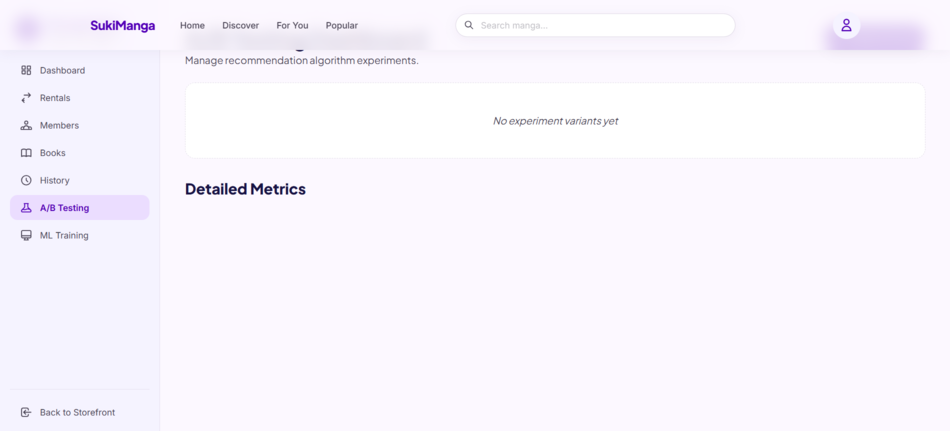
\includegraphics[width=0.8\textwidth]{images/adminABTesting.png}
\caption{หน้าการทดสอบแบบ A/B Testing}
\label{fig:app_adminabtesting}
\end{figure}

% =============================
% ภาคผนวก ข (ตัวอย่าง — uncomment ถ้าต้องการ)
% =============================
% \appendiceschapter{รายละเอียดเพิ่มเติม}
% \section*{หัวข้อ}
% เนื้อหาภาคผนวก ข

% ==========================================
% ประวัติผู้เขียน
% ==========================================
\begin{biography}
% ประวัติผู้เขียน
% หมายเหตุ: ไม่เกิน 1 หน้ากระดาษ
%
% *** ลบข้อความตัวอย่างด้านล่าง แล้วเขียนประวัติของตนเอง ***

\section*{นักศึกษาคนที่ 1}

นายณัฐพัฒน์ แสนตรี เกิดเมื่อวันที่ 01 เมษายน พ.ศ.2547 ที่จังหวัดกาฬสินธุ์
สำเร็จการศึกษาระดับมัธยมศึกษาตอนปลาย จากโรงเรียนสมเด็จพิทยาคม เมื่อปีการศึกษา 2565
ปัจจุบันกำลังศึกษาระดับปริญญาตรี หลักสูตรวิทยาศาสตรบัณฑิต
สาขาวิชาวิทยาการคอมพิวเตอร์ วิทยาลัยการคอมพิวเตอร์ มหาวิทยาลัยขอนแก่น

% ถ้ามีรางวัลหรือทุนการศึกษา:
% ได้รับ ... จาก ... เมื่อ พ.ศ. ...

% ถ้ามีประสบการณ์ทางวิชาการ:
% มีประสบการณ์ ...


% --- uncomment ด้านล่างนี้ ถ้ามีนักศึกษาคนที่ 2 ---
\section*{นักศึกษาคนที่ 2}

นางสาวการติมา คำภีร์ เกิดเมื่อวันที่ 16 มิถุนายน พ.ศ.2547 ที่จังหวัดศรีสะเกษ
สำเร็จการศึกษาระดับมัธยมศึกษาตอนปลาย จากโรงเรียนขุขันธ์ เมื่อปีการศึกษา 2565
ปัจจุบันกำลังศึกษาระดับปริญญาตรี หลักสูตรวิทยาศาสตรบัณฑิต
สาขาวิชาวิทยาการคอมพิวเตอร์ วิทยาลัยการคอมพิวเตอร์ มหาวิทยาลัยขอนแก่น

\end{biography}

\end{document}